\section{Motivation}
\begin{frame}
\frametitle{Applied Topology}
\begin{minipage}{0.45\columnwidth}%
\begin{tikzpicture}[scale=.5]
    \foreach[count=\p] \x / \y in \data {
    \only<3->{
	\begin{pgfonlayer}{ball}
        \fill[gray!50,radius= .8 cm] (\x,\y) circle{};
        \end{pgfonlayer}{ball}
        }
	\node[draw, circle, scale=.25, fill=white](\p) at (\x, \y) {};
    } 
 \end{tikzpicture}
\end{minipage}%
\begin{minipage}{0.55\columnwidth}%
\begin{enumerate}
\item<1->{ Set of points in $\R^2$}
\item<2->{ Looks like an annulus.}
\end{enumerate}
\end{minipage}
\begin{enumerate}
\item[] What is this?
\item[] What does it look like ?
\end{enumerate}
\only<3->{Applied topology about recovering shape from [geometric] data}
\end{frame}
\begin{frame}
  \frametitle{Wherefore topology? }
  \begin{minipage}{.45\textwidth}
  \begin{tikzpicture}[scale=.5]
    \foreach[count=\p] \x / \y in \data {
    	\node[draw, circle, scale=.25, fill=white](\p) at (\x, \y) {};
	\draw[red] (1) -- (100);
	\draw[bend left, green] (1) -- (96) -- (12) -- (28) -- (66) -- (60) -- (89) -- (64) -- (100); 
    } 
 \end{tikzpicture}
  \end{minipage}
  \begin{minipage}{.65\textwidth}
    Geometry is too rigid! \\
    \noindent Trouble with distance metrics:
    \begin{description}
    \item[Unreliable] Only trust small distances
    \item[Ill motivated] The metrics in use may be arbitrarily chosen
    \end{description}
    \end{minipage}
\end{frame}

\begin{frame}
  \frametitle{Wherefore topology? }
  \begin{minipage}{.25\textwidth}
  \begin{tikzpicture}[scale=.5]
    \foreach[count=\p] \x / \y in \data {
	\begin{pgfonlayer}{ball}
        \fill[gray!50,radius= .8 cm] (\x,\y) circle{};
        \end{pgfonlayer}{ball}
	\node[draw, circle, scale=.25, fill=white](\p) at (\x, \y) {};
    } 
 \end{tikzpicture}
  \end{minipage}
  \begin{minipage}{.65\textwidth}
  \begin{description}
      \item Depend only on \emph{nearness}. 
      \item \emph{Count} qualitative features.
      \item Dimension Agnostic.
      \end{description}
    \end{minipage}
    \vfill
\end{frame}

\begin{frame}
\frametitle{Persistent Homology}
TODO: Study how shape changes over scale
\end{frame}

\begin{frame}{Applications of Persistent Homology}
\begin{center}
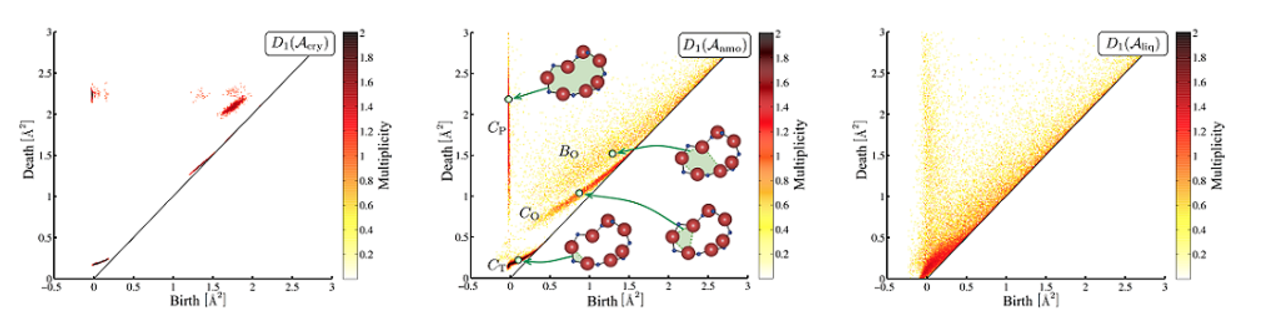
\includegraphics[height=2cm]{persistence_and_materials}
%\caption{Materials Science: of $Si02$ in different amorphous states. Hiraoka}
\end{center}
\begin{minipage}{.43\textwidth}
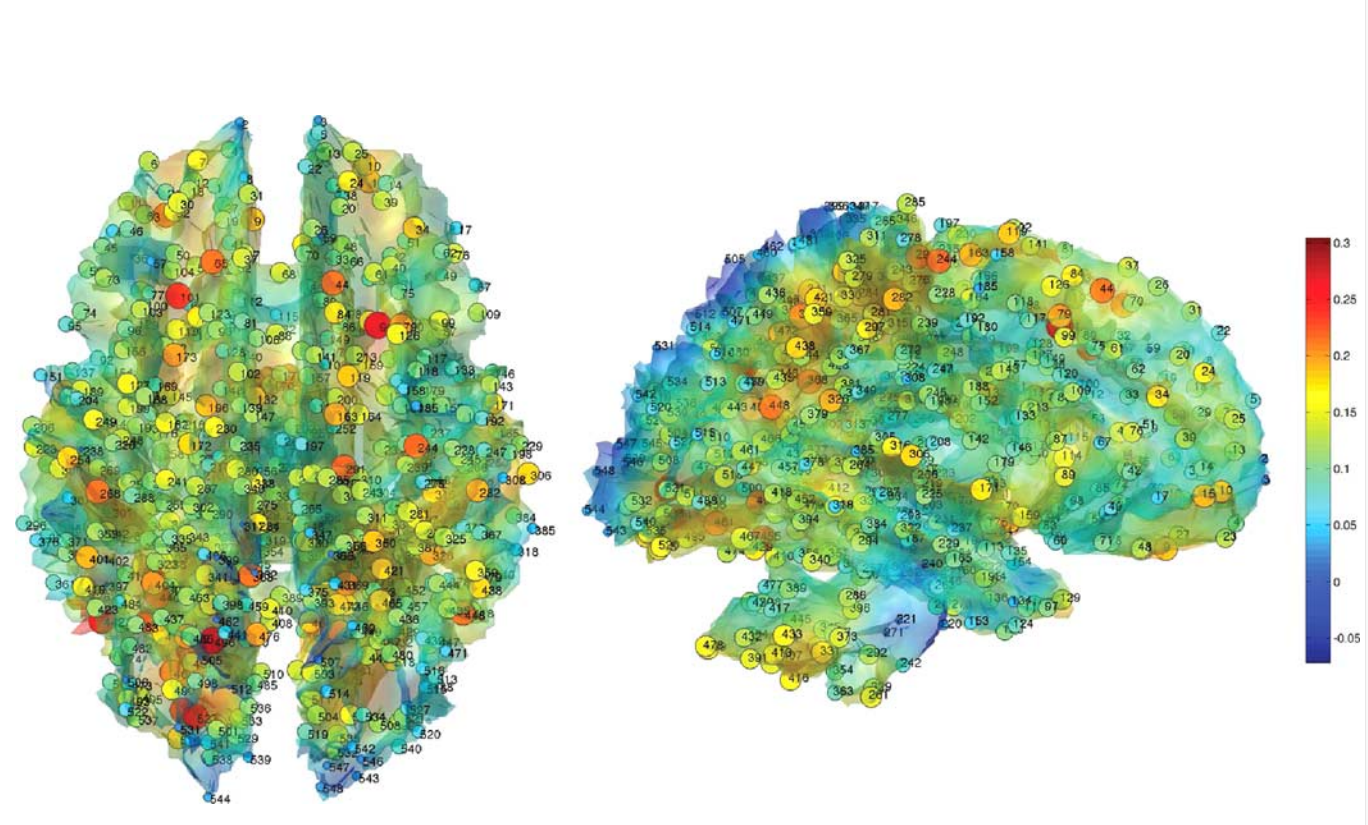
\includegraphics[height=2cm]{complex_on_brains}
%\caption{Brains! Credit: Chung}
%\source{Chung}
\end{minipage}
\begin{minipage}{.43\textwidth}
\hfill
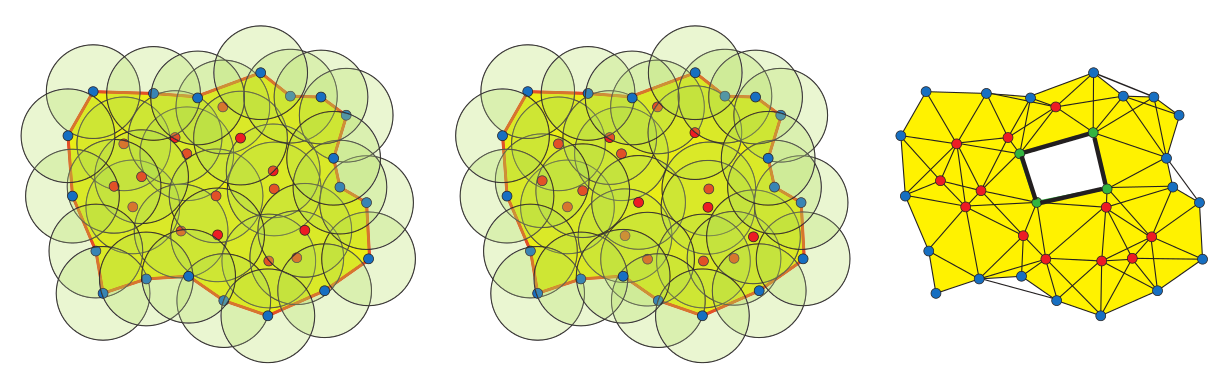
\includegraphics[height=2cm]{sensors}
%\caption{Sensor Networks}
%\source{Ghrist}
\end{minipage}
\pause
\begin{center}
\textbf{Efficient Algorithms Enable Applications}
\end{center}
\end{frame}

